\chapter{势阱、势垒与隧道效应}\label{ch:b2:potential-wells-tunneling}

一个小球在碗中来回滚动，其能量取决于它最初所获得的能量；
原子中的电子、原子核中的核子、纳米尺寸晶体中的电子，
只能取某些特定的能量，其中最低的一个并不为零。
小球无法越过高于其能量所允许的山丘；
$\alpha$ 粒子要离开原子核，须穿过一道它永远无法攀越的库仑壁垒；
扫描隧道显微镜的针尖横跨真空间隙产生电流，
氨分子中的氮原子每秒穿过其三个氢原子所在的平面，
次数高达二百四十亿次。
本章在最简单的势中求解薛定谔方程——
无限深与有限深的势阱、台阶、势垒与双势阱——
并由此得出经典力学无法给出的两个量子事实：
束缚态能量的\emph{量子化}，
以及穿过经典禁区的\emph{\omterm{thm:b2:potential-wells-tunneling:tunnel}{隧道效应}}，
其对势垒宽度与高度呈指数级敏感，
因此它可作为皮米量级的尺子，
也正因此放射性寿命跨越了三十个数量级。

\begin{omfigure}
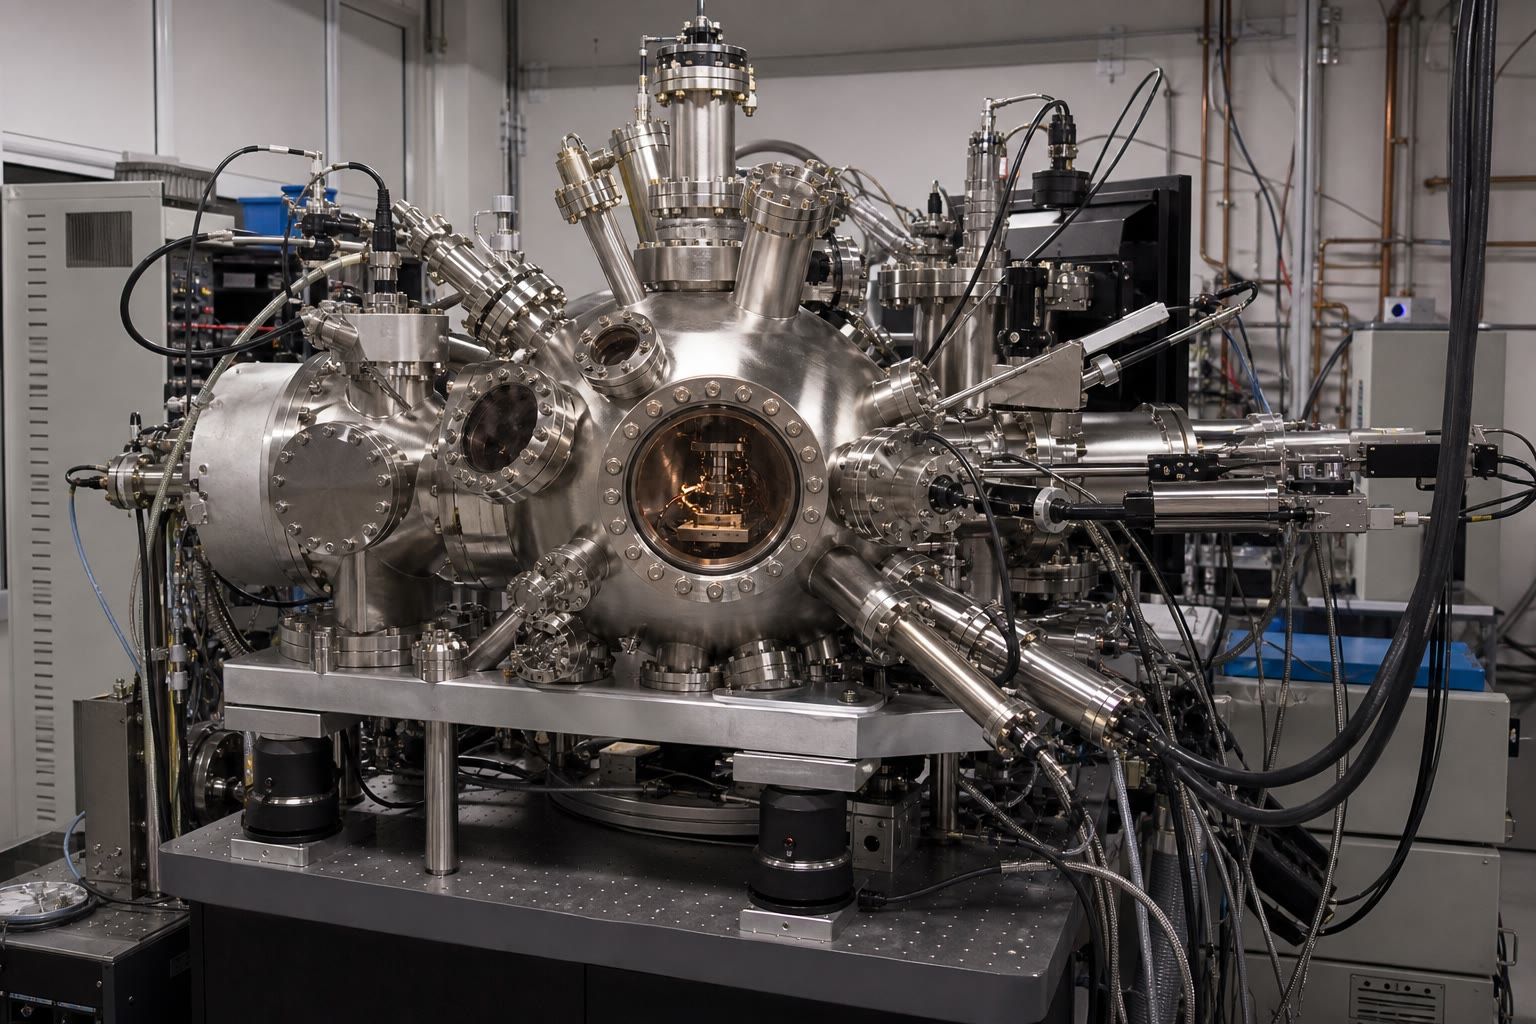
\includegraphics[width=0.58\linewidth]{images/book4/ai/b4-31-stm-instrument.jpg}

{\small 扫描隧道显微镜：金属针尖悬于表面上方零点几纳米处；
隧道电流每变化十分之一纳米即变为原来的十倍，
由此可逐个原子地描绘出表面
形貌。}
\end{omfigure}

\section{无限深势阱}

\begin{proposition}[无限深势阱]\label{prop:b2:potential-wells-tunneling:infinite}
粒子被不可穿透的壁限制在 $0 < x < L$ 内（区域内 $V = 0$，
区域外 $V = \infty$，因此壁上 $\varphi = 0$）。该粒子的
\omterm{thm:b2:schrodinger-wave-functions:stationary}{定态}与能量为
\[
\varphi_n(x) = \sqrt{\frac{2}{L}}\sin\frac{n\pi x}{L}, \qquad
E_n = \frac{n^2h^2}{8mL^2} = n^2E_1, \qquad n = 1, 2, 3, \dots
\]
能量是\emph{量子化的}\index{量子化的}，
随 $n^2$ 增长，且最低能级并不为零：\emph{限域
能}\index{限域能} $E_1 = h^2/8mL^2$ 是
定域化所付出的代价（$\Delta x \sim L$ 要求 $\Delta p \sim h/2L$）。
$\varphi_n$ 两两正交，$\int\varphi_n\varphi_m\dd x = \delta_{nm}$，
且势阱中的任一态都是它们的叠加。
\end{proposition}

\begin{proof}
区域内 $\varphi'' = -k^2\varphi$，其中 $k^2 = 2mE/\hbar^2$：$\varphi = A\sin kx
+ B\cos kx$；由 $\varphi(0) = 0$ 可知 $B$ 为零，由 $\varphi(L) = 0$ 得 $kL = n\pi$，
——这正是弦的驻波，且 $E = \hbar^2k^2/2m$。
归一化给出 $A = \sqrt{2/L}$；正交性即
正弦函数的正交性。
\end{proof}

\begin{omfigure}
\begin{tikzpicture}[scale=0.9]
  \draw[thick] (0,0) -- (0,4.6); \draw[thick] (4,0) -- (4,4.6); \draw[thick] (0,0) -- (4,0);
  \foreach \n/\y/\c in {1/0.45/omDef, 2/1.8/omThm, 3/4.05/omExo}{
    \draw[\c, thick] (0,\y) -- (4,\y);
    \node[font=\scriptsize, \c, right] at (4.1,\y) {$E_\n = \n^2E_1$};
    \draw[\c, thick, domain=0:4, samples=80] plot (\x,{\y+0.35*sin(deg(\n*pi*\x/4))});
  }
  \node[font=\scriptsize] at (2,-0.35) {$0 < x < L$};
  \begin{scope}[xshift=7.5cm]
    \draw[thick] (0,0) -- (0,4.6); \draw[thick] (4,0) -- (4,4.6); \draw[thick] (0,0) -- (4,0);
    \foreach \n/\y/\c in {1/0.45/omDef, 2/1.8/omThm, 3/4.05/omExo}{
      \draw[\c, thick, domain=0:4, samples=80] plot (\x,{\y+0.5*(sin(deg(\n*pi*\x/4)))^2});
      \draw[gray!60, thin] (0,\y) -- (4,\y);
    }
    \node[font=\scriptsize] at (2,-0.35) {$|\varphi_n|^2$};
  \end{scope}
\end{tikzpicture}

{\small 无限深势阱：前三个能级 $E_n \propto n^2$，
及其\omterm{def:b2:schrodinger-wave-functions:psi}{波函数}（左）与概率密度（右）——
波节数为 $n - 1$，基态遍布整个势阱，
且能量不为零。}
\end{omfigure}

\begin{example}[数量级与颜色]\label{ex:b2:potential-wells-tunneling:orders}
$E_1 = h^2/8mL^2$：位于 \qty{1}{nm} 内的电子能量为 \qty{0.38}{eV}；
位于 \qty{0.1}{nm}（原子尺度）内时为 \qty{38}{eV}，这是原子能量的数量级；
位于 \qty{5}{fm} 内的核子为 \qty{8}{MeV}，这是核能的数量级；
处于盒中的弹珠为 $10^{-63}\,\unit{J}$——没有人会察觉。
直径仅几纳米的\omterm{rem:b2:charges-currents-conduction:materials}{半导体}纳米晶体（即\emph{量子
点}）会束缚其中的电子：\omterm{prop:b2:potential-wells-tunneling:infinite}{限域能}会叠加到晶体的能隙上，因此点越小，
发出的光就越偏蓝——同一种材料，
在 \qty{6}{nm} 时发红光，在 \qty{3}{nm} 时发绿光，
仅靠尺寸即可调控。
\end{example}

\section{有限深势阱}

\begin{proposition}[有限深势阱]\label{prop:b2:potential-wells-tunneling:finite}
对于 $V = 0$（$|x| < a$ 内）、$V = V_0$（区域外）时，$0 < E < V_0$ 的态
在区域内振荡（$k = \sqrt{2mE}/\hbar$），在区域外衰减（$\kappa =
\sqrt{2m(V_0 - E)}/\hbar$），墙外 $\varphi \propto \eu^{-\kappa|x|}$。
令 $\varphi$ 与 $\varphi'$ 在 $x = \pm a$ 处连续，于是对偶态与
奇态分别满足：
\[
k\tan ka = \kappa \quad\text{（偶）}, \qquad
-k\cot ka = \kappa \quad\text{（奇）}, \qquad\text{且}\quad
(ka)^2 + (\kappa a)^2 = \frac{2mV_0a^2}{\hbar^2} \equiv R^2 .
\]
图解法中，解即曲线 $\eta =
\xi\tan\xi$、$\eta = -\xi\cot\xi$ 与圆 $\xi^2 + \eta^2 = R^2$ 的
交点（$\xi = ka$，$\eta = \kappa a$）：\emph{总存在至少一个
束缚态}（偶基态），共 $1 + \lfloor 2R/\pi\rfloor$ 个。
粒子会\emph{穿入}禁区，穿入深度为
$1/\kappa$，且各能级均低于同宽
无限深势阱的对应能级。
\end{proposition}

\begin{proof}
偶解在阱内为 $A\cos kx$，阱外为 $B\eu^{-\kappa|x|}$；
由 $\varphi'/\varphi$ 在 $x = a$ 处的连续性，得 $-k\tan ka = -\kappa$。
奇解同理，改用 $\sin$。圆即 $k$ 与
$\kappa$ 的定义。$\xi\tan\xi$ 的各分支，始于 $\xi = n\pi$ 者，与
$-\xi\cot\xi$ 的各分支，始于 $(n + \tfrac12)\pi$ 者，与圆恰交一次，若
其起点在圆内，由此得上述计数。
\end{proof}

\begin{omfigure}
\begin{tikzpicture}
  \begin{axis}[omaxis, width=8.6cm, height=5cm, xmin=0, xmax=5.2, ymin=0, ymax=5.2,
    xlabel={$\xi = ka$}, ylabel={$\eta = \kappa a$}, xtick={1.571,3.142,4.712}, xticklabels={$\pi/2$,$\pi$,$3\pi/2$}, ytick=\empty, clip=true,
    legend style={font=\scriptsize, at={(0.98,0.98)}, anchor=north east, draw=none, fill=white}]
    \addplot[omDef, thick, domain=0:1.5, samples=80] {x*tan(deg(x))};
    \addlegendentry{$\xi\tan\xi$（偶）}
    \addplot[omExo, thick, domain=1.6:3.1, samples=80] {-x/tan(deg(x))};
    \addlegendentry{$-\xi\cot\xi$（奇）}
    \addplot[omDef, thick, domain=3.2:4.65, samples=80] {x*tan(deg(x))};
    \addplot[omExo, thick, domain=4.75:5.2, samples=40] {-x/tan(deg(x))};
    \addplot[omThm, thick, domain=0:4, samples=100] {sqrt(16-x*x)};
    \addlegendentry{$\xi^2 + \eta^2 = R^2$}
    \addplot[gray, dashed, domain=0:1.2, samples=40] {sqrt(1.44-x*x)};
  \end{axis}
\end{tikzpicture}

{\small 有限深阱的图解：束缚态为
半径 $R = a\sqrt{2mV_0}/\hbar$ 的圆与
分支 $\xi\tan\xi$（偶态）、$-\xi\cot\xi$（奇态）的交点。
此处 $R = 4$，故有三个束缚态；虚线小圆（$R = 1.2$）仍与第一支相交，
即阱总至少束缚一个态。}
\end{omfigure}

\begin{example}[纳米阱中的电子]\label{ex:b2:potential-wells-tunneling:finite}
阱深 $V_0 = \qty{1}{eV}$，宽 $2a = \qty{1}{nm}$：$R = a\sqrt{2mV_0}/\hbar = 0.5 \times
10^{-9} \times 5.1 \times 10^9 = 2.6$，故共有 $1 + \lfloor 2R/\pi\rfloor = 2$ 个
束缚态；基态能量在 \qty{0.26}{eV} 附近，而无限深阱的基态能量为
\qty{0.38}{eV}，粒子渗入阱壁约 \qty{0.2}{nm}
（$1/\kappa = \hbar/\sqrt{2m(V_0 - E)}$）。此类阱以
数纳米厚的\omterm{rem:b2:charges-currents-conduction:materials}{半导体}薄层生长而成，是二极管\omterm{def:b2:laser:cavity}{激光器}的核心，
见\cref{ch:b2:laser}。
\end{example}

\section{势阶与势垒：隧道效应}

\begin{proposition}[势阶]\label{prop:b2:potential-wells-tunneling:step}
能量为 $E$ 的粒子自 $x < 0$ 一侧射向台阶 $V = V_0$，
台阶位于 $x > 0$ 区域：
\begin{itemize}
\item $E > V_0$：左侧 $\varphi = \eu^{\iu k_1x} + r\eu^{-\iu k_1x}$，右侧为 $t\eu^{\iu
      k_2x}$，其中 $k_{1,2} = \sqrt{2m(E - V_{0,\text{左/右}})}/
      \hbar$；由 $\varphi$ 与 $\varphi'$ 的连续性得 $r = (k_1 - k_2)/(k_1
      + k_2)$，反射概率（电流之比）为 $R = r^2$，
      $T = 1 - R = 4k_1k_2/(k_1 + k_2)^2$——粒子\emph{可被能量足以攀越的
      台阶反射}，正如弦上的波因阻抗变化而反射
      （见\cref{ch:b2:wave-interfaces}）；
\item $E < V_0$：右侧 $\varphi = t\eu^{-\kappa x}$，$\kappa = \sqrt{2m(V_0
      - E)}/\hbar$——一个\emph{倏逝波}\index{倏逝波 （量子）}
；$|r| = 1$（\omterm{thm:b2:wave-interfaces:snell}{全反射}，伴有相移），
      无电流流入台阶，但粒子在该处被发现的
      概率在 $1/\kappa$ 范围内衰减。
\end{itemize}
\end{proposition}

\begin{proof}
在 $x = 0$ 处写出\omterm{thm:b2:fluid-kinematics:continuity}{连续性方程}并求解；计算电流时
取 $j = (|A|^2 - |B|^2)\hbar k/m$（见\cref{ch:b2:schrodinger-wave-functions}）。
当 $E < V_0$ 时，$r = (k - \iu\kappa)/(k + \iu\kappa)$，模为 1。
\end{proof}

\begin{theorem}[穿过势垒的隧道效应]\label{thm:b2:potential-wells-tunneling:tunnel}
能量为 $E < V_0$ 的粒子遇到一个矩形势垒，其高度为
$V_0$、宽度为 $a$，其透射概率为
\[
T = \Big[1 + \frac{V_0^2\sinh^2(\kappa a)}{4E(V_0 - E)}\Big]^{-1}
\ \approx\ 16\,\frac{E}{V_0}\Big(1 - \frac{E}{V_0}\Big)\eu^{-2\kappa a}
\quad (\kappa a \gg 1), \qquad
\kappa = \frac{\sqrt{2m(V_0 - E)}}{\hbar} .
\]
这就是\emph{隧道效应}\index{隧道效应}：经典上
不可能，量子力学下却指数级地小——并且
对宽度 $a$、高度 $V_0 - E$ 与
质量 $m$ 呈指数级敏感。对于比顶部低 \qty{1}{eV} 的电子，$\kappa = \qty{5.1}{nm^{-1}}$：
$T \sim 10^{-2}$（$a = \qty{0.5}{nm}$），$10^{-4}$ 对应 \qty{1}{nm}，$10^{-9}$ 对应
\qty{2}{nm}；对于质子，$\kappa$ 是前者的 $43$ 倍，在这些宽度下
几乎无法穿过。
\end{theorem}

\begin{proof}
$\varphi = \eu^{\iu kx} + r\eu^{-\iu kx}$（$x < 0$）；势垒内为 $A\eu^{\kappa x} + B\eu^{-\kappa x}$，
$t\eu^{\iu kx}$（$x > a$）；四个连续性条件（$\varphi$ 与
$\varphi'$ 在 $0$、$a$ 处）共四个未知数；消去 $A$、$B$、$r$，
得 $1/|t|^2 = 1 + (k^2 + \kappa^2)^2\sinh^2(\kappa a)/4k^2\kappa^2$，即为上式，其中
$k^2 = 2mE/\hbar^2$，$\kappa^2 = 2m(V_0 - E)/\hbar^2$。当
$\kappa a \gg 1$ 时，$\sinh\kappa a \approx \eu^{\kappa a}/2$。对形状任意的
势垒，指数项变为 $2\int\kappa(x)\dd x$，积分沿
整个禁区进行，即伽莫夫因子，在本阶段不加证明地承认。
\end{proof}

\begin{omfigure}
\begin{tikzpicture}[scale=0.9, >=stealth]
  \fill[gray!15] (3,0) rectangle (4.2,2.6);
  \draw[thick] (0,0) -- (3,0) -- (3,2.6) -- (4.2,2.6) -- (4.2,0) -- (7.5,0);
  \draw[dashed, omExo] (0,1.2) -- (7.5,1.2) node[right, font=\scriptsize] {$E$};
  \node[font=\scriptsize] at (3.6,2.85) {$V_0$};
  \draw[<->, thin] (3,-0.3) -- (4.2,-0.3) node[midway, below, font=\scriptsize] {$a$};
  % wave: incident+reflected (left), evanescent (inside), transmitted (right)
  \draw[omDef, thick, domain=0:3, samples=120] plot (\x,{1.2+0.5*cos(deg(6*\x))});
  \draw[omDef, thick, domain=3:4.2, samples=40] plot (\x,{1.2+0.5*exp(-1.6*(\x-3))});
  \draw[omDef, thick, domain=4.2:7.5, samples=120] plot (\x,{1.2+0.073*cos(deg(6*(\x-4.2)))});
  \node[font=\scriptsize, omDef] at (1.5,2.1) {$\eu^{\iu kx} + r\eu^{-\iu kx}$};
  \node[font=\scriptsize, omDef] at (3.6,1.95) {$\eu^{-\kappa x}$};
  \node[font=\scriptsize, omDef] at (6.0,1.75) {$t\eu^{\iu kx}$, $|t|^2 \approx 16\frac{E}{V_0}(1 - \frac{E}{V_0})\eu^{-2\kappa a}$};
\end{tikzpicture}

{\small 隧穿势垒：波在左侧振荡，
在经典禁戒区域内指数衰减，并且
在右侧以减小的振幅射出——波长相同，
概率很小。}
\end{omfigure}

\begin{example}[扫描隧道显微镜]\label{ex:b2:potential-wells-tunneling:stm}
将一根尖锐的金属探针靠近导电表面，二者间距 $d \approx \qty{0.5}{nm}$，
并施加一小电压：电子穿过真空间隙隧穿，
势垒高度即逸出功 $\Phi \approx
\qty{4.5}{eV}$，于是 $\kappa = \sqrt{2m\Phi}/\hbar = \qty{1.1e10}{m^{-1}}$，
电流 $I \propto \eu^{-2\kappa d}$ 每 \qty{0.1}{nm} 改变 $\eu^{2.2} \approx
10$ 倍。\omterm{def:b2:feedback-oscillators:loop}{反馈}回路移动探针以保持 $I$
不变，探针扫描时记录的高度描绘出表面，
竖直分辨率可达皮米量级——横向则可逐个原子分辨，
因为探针末端最靠近表面的那个原子承载了大部分
电流（宾尼希与罗雷尔，1981）。
\end{example}

\begin{example}[α 衰变]\label{ex:b2:potential-wells-tunneling:alpha}
重原子核内能量为 \qty{5}{MeV} 的 $\alpha$ 粒子，面对
剩余电荷 $Ze$ 产生的库仑势垒，在核表面处高达数十 MeV，
并延伸至半径 $b = 2Ze^2/4\pi\varepsilon_0E
\approx \qty{50}{fm}$ 处，此处 $V = E$。伽莫夫因子 $2\int\kappa\,\dd r$
数量级为 $80$：$T \sim \eu^{-80} \sim 10^{-35}$。粒子撞击势垒内壁
每秒约 $10^{21}$ 次，因此以 $\sim 10^{-14}
\,\unit{s^{-1}}$ 的速率逃逸——寿命约为一百万年。由于指数
随 $Z/\sqrt E$ 变化，$\qty{2}{MeV}$ 的 $E$ 变化使寿命
改变二十个数量级——盖革–纳托尔定律，
从微秒到宇宙年龄不等（伽莫夫，1928 年：
\omterm{thm:b2:potential-wells-tunneling:tunnel}{隧道效应}的首次应用）。
\end{example}

\begin{omfigure}
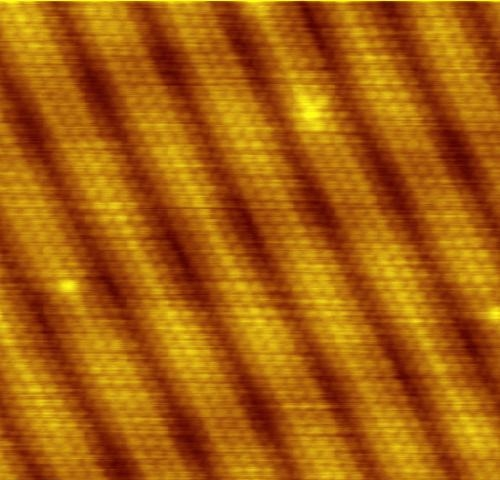
\includegraphics[width=0.42\linewidth]{images/book4/stm-gold-100.jpg}

{\small 金表面的原子分辨图像，由扫描隧道显微镜拍摄：重构 (100) 面上的原子列，相隔约十分之几纳米。}
\end{omfigure}

\section{双势阱}

\begin{proposition}[隧道劈裂]\label{prop:b2:potential-wells-tunneling:double}
两个相同的势阱被一个势垒隔开：若势垒不可穿透，
则每个势阱都有相同的基能级 $E_0$，共两个。
隧穿使两者耦合，双势阱的两个最低态为
\emph{对称}与\emph{反对称}的组合，
$\varphi_\pm \approx (\varphi_{\text{L}} \pm \varphi_{\text{R}})/\sqrt2$，能量为
$E_0 \mp \Delta/2$：能级被\emph{劈裂}，劈裂量 $\Delta \propto
\eu^{-\kappa a}$（为隧穿振幅，而非其平方）。粒子
置于左势阱中，$\psi = (\varphi_+ + \varphi_-)/\sqrt2$，并不
处于\omterm{thm:b2:schrodinger-wave-functions:stationary}{定态}：它以频率
$\nu = \Delta/h$——\emph{隧穿振荡}，
即\cref{ch:b2:schrodinger-wave-functions}中的双能级拍。
\end{proposition}

\begin{proof}
对称组合在势垒下没有节点，并且
曲率较小，因而能量较低；反对称组合有一个节点，
能量较高；劈裂量正比于势垒下局域函数的
交叠，即 $\eu^{-\kappa a}$。拍
就是前面已算过的双能级叠加。
\end{proof}

\begin{omfigure}
\begin{tikzpicture}[scale=0.9]
  % double well potential
  \draw[thick] (0,3) -- (0,0) -- (1.8,0) -- (1.8,1.6) -- (2.4,1.6) -- (2.4,0) -- (4.2,0) -- (4.2,3);
  \draw[omDef, thick] (0,0.7) -- (4.2,0.7); \node[font=\scriptsize, omDef, right] at (4.3,0.62) {$E_0 - \Delta/2$};
  \draw[omExo, thick] (0,1.0) -- (4.2,1.0); \node[font=\scriptsize, omExo, right] at (4.3,1.08) {$E_0 + \Delta/2$};
  \begin{scope}[xshift=7.2cm]
    \draw[thick] (0,3) -- (0,0) -- (1.8,0) -- (1.8,1.6) -- (2.4,1.6) -- (2.4,0) -- (4.2,0) -- (4.2,3);
    \draw[omDef, thick, domain=0:1.8, samples=50] plot (\x,{2.2+0.5*sin(deg(pi*\x/1.8))});
    \draw[omDef, thick] (1.8,2.2) .. controls (2.0,2.27) and (2.2,2.27) .. (2.4,2.2);
    \draw[omDef, thick, domain=2.4:4.2, samples=50] plot (\x,{2.2+0.5*sin(deg(pi*(\x-2.4)/1.8))});
    \node[font=\scriptsize, omDef, right] at (4.3,2.3) {$\varphi_+$ 对称};
    \draw[omExo, thick, domain=0:1.8, samples=50] plot (\x,{0.9+0.5*sin(deg(pi*\x/1.8))});
    \draw[omExo, thick] (1.8,0.9) .. controls (2.0,0.83) and (2.2,0.97) .. (2.4,0.9);
    \draw[omExo, thick, domain=2.4:4.2, samples=50] plot (\x,{0.9-0.5*sin(deg(pi*(\x-2.4)/1.8))});
    \node[font=\scriptsize, omExo, right] at (4.3,0.9) {$\varphi_-$ 反对称};
  \end{scope}
\end{tikzpicture}

{\small 双势阱：两个孤立势阱的简并能级
劈裂为对称态（较低）与反对称态（较高），
劈裂量 $\Delta \propto \eu^{-\kappa a}$；粒子从一侧出发，
以频率 $\Delta/h$ 来回隧穿。}
\end{omfigure}

\begin{example}[氨分子]\label{ex:b2:potential-wells-tunneling:ammonia}
在 NH$_3$ 中，氮原子位于三个氢原子所在平面的
一侧或另一侧——这是一个势垒约为
\qty{0.25}{eV} 的双势阱。基能级的隧道劈裂为 $\Delta =
\qty{1e-4}{eV}$：$\nu = \Delta/h = \qty{24}{GHz}$，即\emph{反转}
频率，即第一台微波激射器与第一台原子钟所用的
跃迁（1949 年）。若将氢换成氘，较重的分子
隧穿得更少：\qty{1.6}{GHz}。在更重的类锥形分子（PH$_3$、AsH$_3$）中，
劈裂缩减至千赫兹甚至更低：分子
会在同一侧停留数年之久——这正是左旋与右旋分子
得以存在的原因，也是糖在架上不会消旋的原因。
\end{example}

\begin{omfigure}
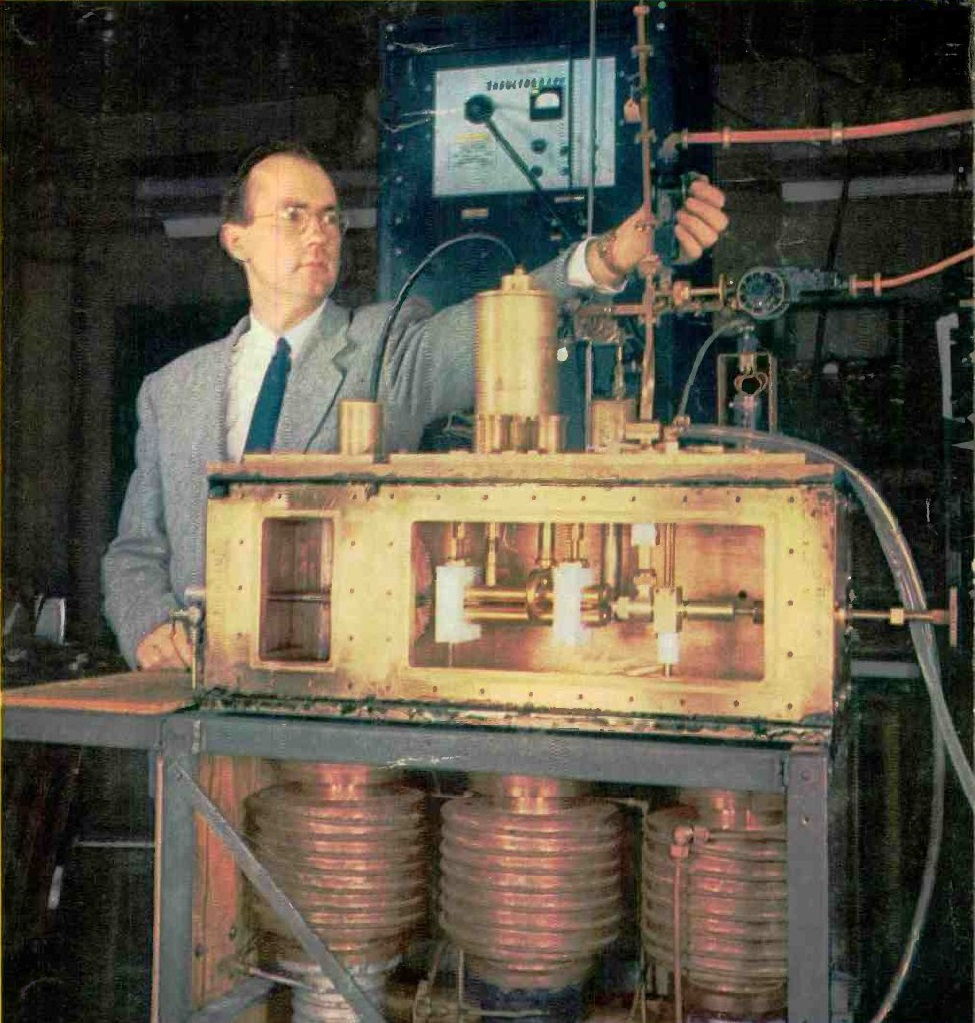
\includegraphics[width=0.5\linewidth]{images/book4/townes-maser.jpg}

{\small 查尔斯·汤斯与第一台微波激射器（1954 年）：经电场分拣进入上反转态的氨分子束，在谐振腔中放大了 \qty{24}{GHz} 的跃迁——这是\omterm{def:b2:laser:processes}{受激辐射}的首个器件，比激光早六年。}
\end{omfigure}

\begin{method}[势阱与势垒]\label{meth:b2:potential-wells-tunneling:method}
(1) 分区域写出 $\varphi$：$\eu^{\pm\iu kx}$ 用于 $E > V$ 的区域，
$\eu^{\pm\kappa x}$ 用于 $E < V$ 的区域，其中 $k, \kappa = \sqrt{2m|E - V|}/\hbar$。
(2) 在每个边界处匹配 $\varphi$ 与 $\varphi'$（在无限高壁处，
$\varphi = 0$）。(3) 束缚态：匹配条件仅对离散的
$E$ 有解——用图解法计数。(4) 散射：流
密度 $(|A|^2 - |B|^2)\hbar k/m$ 给出 $R$ 与 $T$。(5) 隧穿：$T \sim
\eu^{-2\kappa a}$；先估数量级，再求前置因子。(6)
双势阱：劈裂 $\propto\eu^{-\kappa a}$，拍频为 $\Delta/h$。
\end{method}

\section{练习}

\begin{exercise}[$\star$]\label{exo:b2:potential-wells-tunneling:1}
无限深势阱：宽 \qty{1}{nm} 的阱中电子（$E_1$、$E_2$、$E_3$、
$2 \to 1$ 光子的波长）；宽 \qty{0.1}{nm} 的阱中电子；宽 \qty{5}{fm} 的阱中核子；
一颗 \qty{1}{g} 的弹珠在 \qty{10}{cm} 宽的阱中（$E_1$，以及速率为
\qty{1}{cm/s} 时的量子数）。
\end{exercise}

\begin{exercise}[$\star$]\label{exo:b2:potential-wells-tunneling:2}
量子点：带隙为 \qty{1.74}{eV} 的纳米晶体束缚一个电子–空穴对，
其\omterm{prop:b2:potential-wells-tunneling:infinite}{限域能}为 $h^2/8m^*L^2$，其中
$m^* = 0.1\,m_{\text{e}}$。求 $L = 6$、$4$、$3$、
\qty{2.5}{nm} 时的发射波长，各为何色？
\end{exercise}

\begin{exercise}[$\star$]\label{exo:b2:potential-wells-tunneling:3}
隧穿：$V_0 - E = \qty{4.5}{eV}$ 的电子：求 $\kappa$；$\eu^{-2\kappa a}$
在 $a = 0.3$、$0.5$、$1$、\qty{2}{nm} 时的值；每 \qty{0.1}{nm} 的因子；同样
对质子在 $a = \qty{0.3}{nm}$ 时计算。
\end{exercise}

\begin{exercise}[$\star$]\label{exo:b2:potential-wells-tunneling:4}
阶跃势：能量为 \qty{2}{eV} 的电子射向高 \qty{1}{eV} 的台阶：求 $k_1$、$k_2$、
$R$、$T$。对下降 \qty{1}{eV} 的台阶做同样计算；为何经典上不可能，
光学中的类比是什么？
\end{exercise}

\begin{exercise}[$\star\star$]\label{exo:b2:potential-wells-tunneling:5}
\emph{无限深势阱细节。}(a) 求能级并归一化。
(b) 证明正交性。(c) 对 $n = 1$，求 $\langle x\rangle$、$\Delta x =
L\sqrt{1/12 - 1/2\pi^2}$、$\langle p\rangle = 0$、$\Delta p = \pi\hbar/L$，并验证
海森堡不确定关系。(d) 画出 $|\varphi_n|^2$ 在 $n$ 很大时的草图，并与
经典弹跳粒子被找到的概率作比较。
\end{exercise}

\begin{exercise}[$\star\star$]\label{exo:b2:potential-wells-tunneling:6}
\emph{有限深势阱。}(a) 对偶宇称态推导 $k\tan ka = \kappa$。
(b) 用图解法证明总存在束缚态，并对
$R = 1$、$4$、$10$ 计数束缚态个数。(c) 电子，$V_0 = \qty{1}{eV}$，$2a = \qty{1}{nm}$：求
$R$、态数，以及基态的穿透深度（取
$E \approx \qty{0.26}{eV}$）。(d) 束缚态个数
在 $V_0 \to \infty$ 时如何变化，其能量又如何变化？
\end{exercise}

\begin{exercise}[$\star\star$]\label{exo:b2:potential-wells-tunneling:7}
\emph{台阶，$E < V_0$。}(a) 分别写出两侧的 $\varphi$，并求 $r =
(k - \iu\kappa)/(k + \iu\kappa)$。(b) 证明 $|r| = 1$，并求 $r$ 的相位。
(c) 证明 $x > 0$ 时电流为零，尽管该处 $|\varphi|^2 \ne
0$。(d) 电子能量比顶部低 \qty{1}{eV}：求穿透深度；
与\omterm{thm:b2:wave-interfaces:snell}{全反射}的\omterm{def:b2:dispersion-wave-packets:complex}{倏逝波}作比较。
\end{exercise}

\begin{exercise}[$\star\star$]\label{exo:b2:potential-wells-tunneling:8}
\emph{势垒。}(a) 写出四个连续性条件，并
推导 $T$。(b) 对 $E =
V_0/2$、$\kappa a = 3$ 以及 $\kappa a = 1$，分别精确计算并用近似公式计算。(c) 当 $E > V_0$ 时，证明 $T = [1 +
V_0^2\sin^2(k_2a)/4E(E - V_0)]^{-1}$，并求
完全透射的能量。(d) 解释这些能量的物理意义（可参考
在\cref{ch:b2:wave-interfaces}中的增透层）。
\end{exercise}

\begin{exercise}[$\star\star$]\label{exo:b2:potential-wells-tunneling:9}
\emph{伽莫夫。}对从核半径 $R_{\text{n}}$
到 $b = 2Ze^2/4\pi\varepsilon_0E$ 的库仑势垒，指数为 $G = 2\int\kappa\,\dd r =
(2\sqrt{2mE}/\hbar)\,b\,[\arccos\sqrt{R_{\text{n}}/b} - \sqrt{(R_{\text{n}}/b)(1 -
R_{\text{n}}/b)}]$。(a) 设 $Z = 90$，$E = \qty{5}{MeV}$，$R_{\text{n}} = \qty{8}{fm}$，求
$b$、$G$、$T$。(b) 撞击频率 $v/2R_{\text{n}}$ 及其寿命。(c)
对 $E = 4$ 与 \qty{6}{MeV} 重复上述计算，求寿命之比。(d) 为何原子核发射 $\alpha$ 粒子
而非质子或 $^{12}$C？
\end{exercise}

\begin{exercise}[$\star\star\star$]\label{exo:b2:potential-wells-tunneling:10}
\emph{氨分子。}能级劈裂 $\Delta = \qty{1e-4}{eV}$。(a) 求反转频率
以及隧穿振荡的周期。(b) N 原子
初始时制备在一侧：写出 $\psi(t)$，并求
在另一侧找到它的概率。(c) ND$_3$ 的隧穿频率为 \qty{1.6}{GHz}：求 $\kappa a$，
由劈裂之比推出，设 $\Delta \propto \eu^{-\kappa a}$ 且 $\kappa
\propto\sqrt m$（$m_{\text{D}} = 2m_{\text{H}}$，势垒不变）。(d) 为何
手性分子能保持左旋数年之久？
\end{exercise}

\begin{exercise}[$\star\star\star$]\label{exo:b2:potential-wells-tunneling:11}
\emph{扫描隧道显微镜。}$\Phi = \qty{4.5}{eV}$，$d = \qty{0.5}{nm}$，偏压 \qty{0.1}{V}，
$I = \qty{1}{nA}$。(a) 求 $\kappa$、每 \qty{0.1}{nm} 时 $I$ 的变化因子，以及
$I$ 测量精度为 $1\%$ 时的高度分辨率。(b) 电流中每秒
流过的电子数。(c) 针尖顶端原子比其
近邻原子近 \qty{0.25}{nm}（横向相距 \qty{0.25}{nm}，故 $d' = \sqrt{d^2 + 0.25^2}$）：求其
承载电流的比例。(d) 一根 \qty{1}{cm} 的钢框架，
受热后膨胀 $\alpha L\Delta T$，其中 $\alpha = \qty{1e-5}{K^{-1}}$：需要怎样的温度
稳定性才能达到皮米精度？设计上又如何绕开？
\end{exercise}

\begin{exercise}[$\star\star\star$]\label{exo:b2:potential-wells-tunneling:12}
\emph{量子阱\omterm{def:b2:laser:cavity}{激光器}。}一层 \qty{10}{nm} 厚的 GaAs（带隙
\qty{1.42}{eV}，$m_{\text{e}}^* = 0.067\,m_{\text{e}}$，$m_{\text{h}}^* = 0.45\,m_{\text{e}}$）
夹在比阱高 \qty{0.3}{eV} 的势垒之间。(a) 求电子与空穴的
基态\omterm{prop:b2:potential-wells-tunneling:infinite}{限域能}（无限深势阱）。(b) 求激光的光子能量与
波长。(c) 求波长为 \qty{780}{nm} 时的阱宽。(d) 考虑有限高势垒，
该 \qty{10}{nm} 阱中能容纳多少个束缚电子态？
\end{exercise}

\section{周末问题：扫描隧道显微镜、α 粒子与氨分子微波激射器}

\begin{problem}[{周末问题——三次隧穿}]\label{pb:b2:potential-wells-tunneling:1}
数据：$\hbar = \qty{1.05e-34}{J.s}$，$h = \qty{6.63e-34}{J.s}$，$m_{\text{e}} =
\qty{9.11e-31}{kg}$，$m_\alpha = \qty{6.64e-27}{kg}$，$e^2/4\pi\varepsilon_0 =
\qty{1.44}{MeV.fm}$，\qty{1}{eV} $= \qty{1.60e-19}{J}$。

\textbf{第一部分——扫描隧道显微镜。}
针尖与样品均为钨（$\Phi = \qty{4.5}{eV}$）；间隙 $d$；偏压
\qty{50}{mV}；电流为 $I = I_0\eu^{-2\kappa d}$。
\begin{enumerate}
  \item 求费米能级处电子的 $\kappa$，
        该电子面对真空势垒 $\Phi$。
  \item 求 $I$ 的变化因子：$\Delta d = \qty{0.1}{nm}$ 时的值；
        以及 \qty{1}{pm} 时的值。
  \item \omterm{def:b2:feedback-oscillators:loop}{反馈}将 $I$ 保持恒定至 $1\%$：求高度噪声。
  \item 当 $I = \qty{1}{nA}$ 时，求每秒电子数，以及两个电子之间的平均时间间隔，
        并与隧穿“时间” $\sim\hbar/\Phi$ 作比较。
  \item 针尖顶端原子与其近邻原子横向相距 \qty{0.25}{nm}，
        $d = \qty{0.5}{nm}$：求顶端原子所占的份额；为何单个原子
        即可对原子成像。
  \item 吸附原子高 \qty{0.1}{nm}：求恒高模式下 $I$ 的
        变化；为何更倾向于采用恒流模式？
  \item 一根 \qty{2}{cm} 的金属框架，$\alpha = \qty{1e-5}{K^{-1}}$：求使
        针尖移动 \qty{1}{pm} 的温度变化量；仪器如何应对
        （对称性、速度、低膨胀材料）？
  \item 偏压为 \qty{1}{V} 时，势垒不再是矩形：
        画出草图，并判断 $I$ 随 $V$ 的增长是快于还是慢于
        线性增长。
  \item 在氧化的区域上，逸出功为 \qty{3}{eV}，而非
        \qty{4.5}{eV}：在恒流模式下，针尖
        在完全平整的表面上应后撤多少？那么
        STM 图像显示什么？
\end{enumerate}

\textbf{第二部分——原子核 $Z = 92$、$A = 238$ 的 α 衰变。}
$\alpha$ 粒子（$E = \qty{4.2}{MeV}$）在半径为
$R_{\text{n}} = \qty{8}{fm}$ 的原子核中运动；核外库仑势能为 $V(r) =
2(Z - 2)e^2/4\pi\varepsilon_0r$.
\begin{enumerate}[resume]
  \item 势垒在 $R_{\text{n}}$ 处的高度；经典转折点
        $b$。
  \item 核内 $\alpha$ 粒子的速率及其
        撞击核壁的频率。
  \item 伽莫夫指数 $G = (2\sqrt{2mE}/\hbar)\,b\,[\arccos\sqrt{R_{\text{n}}/b}
        - \sqrt{(R_{\text{n}}/b)(1 - R_{\text{n}}/b)}]$ 且 $T = \eu^{-G}$。
  \item 衰变率与半衰期；与实测的 $4.5 \times
        10^9$ 年相比较。
  \item 取 $E = \qty{5.2}{MeV}$（另一同位素）时：半衰期；
        盖革–纳托尔灵敏度。
  \item 取 $R_{\text{n}} = \qty{9}{fm}$（而非 \qty{8}{fm}）时，对
        半衰期的影响；评论此类估算的精度。
  \item 为什么质子（电荷 $1$，质量 $1/4$）的\omterm{thm:b2:potential-wells-tunneling:tunnel}{隧道效应}在同一原子核中
        未被观测到，而 $^{12}$C
        （电荷 $6$）的\omterm{thm:b2:potential-wells-tunneling:tunnel}{隧道效应}是否也未被观测到？
  \item $\alpha$ 粒子以完整的 \qty{4.2}{MeV} 射出，尽管它
        “穿过”了 \qty{30}{MeV} 的势垒：能量是否守恒？
\end{enumerate}

\textbf{第三部分——氨分子激射器。}
氮原子穿过 H$_3$ 平面隧穿；基态能级
分裂量为 $\Delta = \qty{9.8e-5}{eV}$。
\begin{enumerate}[resume]
  \item 反转跃迁的频率与波长。
  \item 用“N 向上”与“N 向下”写出对称态与反对称态；
        哪一个能级更低？为什么？
  \item 制备为“N 向上”的分子：$\psi(t)$，
        时刻 $t$ 处“向下”的概率，以及周期。
  \item 在 \qty{300}{K} 下两能级的玻尔兹曼比：热布居
        能否给出激射？反转如何获得
        （用选态电场）？
  \item 以焦耳计的光子能量；每秒必须发射的分子数，
        使输出功率为 \qty{1e-10}{W}。
  \item ND$_3$ 在 \qty{1.6}{GHz} 处隧穿：求 $\kappa a$，
        对 NH$_3$，假设 $\Delta \propto \eu^{-\kappa a}$ 且 $\kappa \propto \sqrt{m}$。
  \item 该激射器是第一台原子钟：为什么隧穿频率适合作时钟，
        哪些效应会使其发生偏移？
  \item 总结：由限域得到量子化，由倏逝得到隧穿，
        以及由什么确定指数。
\end{enumerate}
\end{problem}
